% ==========================================================================
% G05: Melanoma Detection (PURPLE)
% ==========================================================================
\section{G05}
\setbeamercolor{structure}{fg=violet} % Set G05 Color

\begin{frame}[plain]
\frametitle{G05: Melanoma Detection using Knowledge Distillation}
\begin{columns}[T,totalwidth=\textwidth]
  \begin{column}{0.58\textwidth}
    \textbf{\large Research Question}
    \begin{itemize}
      \item Can Knowledge Distillation compress large CNNs for mobile melanoma screening while maintaining clinical-grade accuracy?
      \item How do temperature and distillation weight affect performance?
    \end{itemize}
    \vspace{0.3cm}
    \textbf{\large Dataset: HAM10000}
    \begin{itemize}
      \item 10,015 dermoscopic images (7,012 train / 1,502 val / 1,513 test)
      \item Binary: Melanoma (11.4\%) vs Non-Melanoma (88.6\%)
      \item Lesion-aware splitting to prevent data leakage
    \end{itemize}
    \vspace{0.3cm}
    \textbf{\large Best Teacher: EfficientNet-B1}
    \begin{table}
      \centering \small
      \begin{tabular}{lccc}
        \toprule
        \textbf{Model} & \textbf{ROC-AUC} & \textbf{ECE} & \textbf{Size (MB)} \\
        \midrule
        EfficientNet-B1 & 0.919 & 0.174 & 25.1 \\
        ResNet-18 & 0.900 & 0.195 & 42.7 \\
        \bottomrule
      \end{tabular}
    \end{table}
  \end{column}
  \begin{column}{0.40\textwidth}
    \begin{figure}
      \centering
      \includegraphics[width=0.95\linewidth]{artifacts/imgs/00_eda/class_distribution.png}
      \caption{\scriptsize HAM10000 class imbalance}
    \end{figure}
  \end{column}
\end{columns}
\end{frame}

\begin{frame}[plain]
\frametitle{Deep Learning Solution: KD + Quantization}
\begin{columns}[T,totalwidth=\textwidth]
  \begin{column}{0.58\textwidth}
    \textbf{\large Methodology}
    \begin{itemize}
      \item \textbf{Teacher:} EfficientNet-B1 (Focal loss, $\gamma$=2, $\alpha$=0.75)
      \item \textbf{Student:} MobileNetV3-Small (9.1 MB, 2.5M params)
      \item \textbf{KD Loss:} $\mathcal{L}_{KD} = \alpha T^2 \text{KL} + (1-\alpha) \mathcal{L}_{\text{focal}}$
      \item \textbf{Optimizer:} AdamW, lr=$10^{-4}$, cosine annealing
    \end{itemize}
    \vspace{0.3cm}
    \textbf{\large Ablation Study}
    \begin{table}
      \centering \scriptsize
      \begin{tabular}{lcccc}
        \toprule
        \textbf{Config} & \textbf{AUC} & \textbf{F1} & \textbf{Recall} & \textbf{ECE} \\
        \midrule
        \textbf{T=1, $\alpha$=0.5} & \textbf{0.921} & \textbf{0.642} & 0.750 & 0.072 \\
        T=1, $\alpha$=0.9 & 0.916 & 0.607 & 0.692 & \textbf{0.064} \\
        T=2, $\alpha$=0.5 & 0.920 & 0.561 & \textbf{0.849} & 0.134 \\
        T=2, $\alpha$=0.9 & 0.919 & 0.556 & 0.843 & 0.130 \\
        \bottomrule
      \end{tabular}
    \end{table}
  \end{column}
  \begin{column}{0.40\textwidth}
    \begin{figure}
      \centering
      \includegraphics[width=0.95\linewidth]{artifacts/imgs/kd_img.png}
      \caption{\scriptsize Knowledge Distillation Framework}
    \end{figure}
  \end{column}
\end{columns}
\end{frame}

\begin{frame}[plain]
\frametitle{Results and Discussion}
\begin{columns}[T,totalwidth=\textwidth]
  \begin{column}{0.58\textwidth}
    \textbf{\large Model Comparison}
    \begin{table}
      \centering \small
      \begin{tabular}{lcccc}
        \toprule
        \textbf{Model} & \textbf{AUC} & \textbf{Acc} & \textbf{ECE} & \textbf{Size} \\
        \midrule
        Teacher (B1) & 0.919 & 86.4\% & 0.174 & 25.1 MB \\
        \textbf{Student} & \textbf{0.921} & \textbf{90.5\%} & \textbf{0.072} & \textbf{9.1 MB} \\
        \midrule
        \multicolumn{2}{l}{\textbf{Compression}} & \multicolumn{2}{c}{2.8$\times$ smaller} & 2.9$\times$ faster \\
        \bottomrule
      \end{tabular}
    \end{table}
    \vspace{0.2cm}
    \textbf{\large Key Findings}
    \begin{itemize}
      \item Student \textbf{exceeds teacher} ROC-AUC (0.921 vs 0.919)
      \item Best config: $T$=1, $\alpha$=0.5 (contrary to $T \geq 3$ convention)
      \item Student correct 67\% when models disagree
      \item 29 shared false negatives (17\% of melanomas)---hard cases
    \end{itemize}
  \end{column}
  \begin{column}{0.40\textwidth}
    \begin{figure}
      \centering
      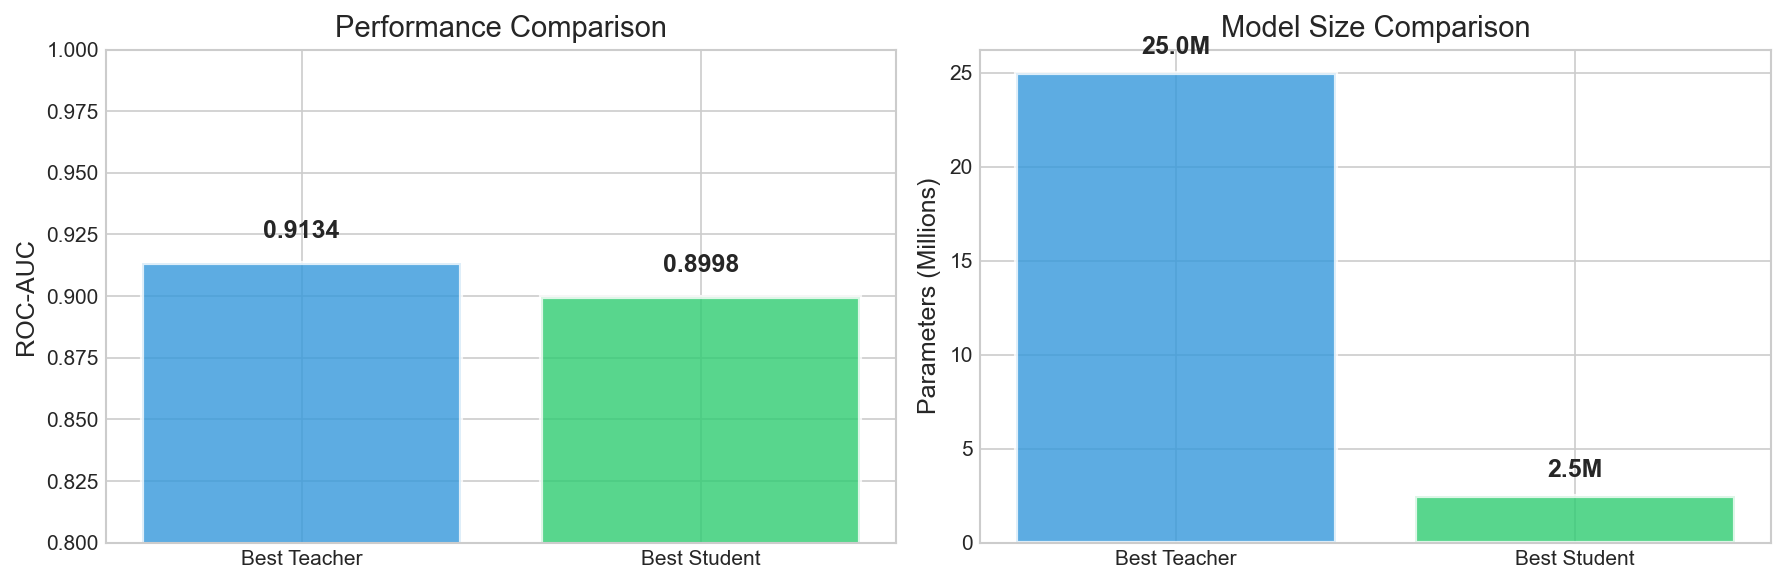
\includegraphics[width=0.95\linewidth]{artifacts/imgs/01_baselines/kd_effectiveness.png}
      \caption{\scriptsize Student vs Teacher Performance}
    \end{figure}
  \end{column}
\end{columns}
\end{frame}
